\documentclass[10pt]{article}
\usepackage[utf8]{inputenc}
\usepackage[T1]{fontenc}
\usepackage{amsmath}
\usepackage{amsfonts}
\usepackage{amssymb}
\usepackage[version=4]{mhchem}
\usepackage{stmaryrd}
\usepackage{graphicx}
\usepackage[export]{adjustbox}
\graphicspath{ {./images/} }

\begin{document}
\begin{center}
\begin{tabular}{|l|l|}
\hline
Convert $\frac{4 \pi}{9}$ to degrees (1 point) & Convert $600^{\circ}$ to radians ( 1 point) \\
\hline
\multicolumn{2}{|l|}{Find two coterminal angles (one positive and one negative) for $\frac{3 \pi}{7}$ (1 point each)} \\
\hline
Positive & Negative \\
\hline
\multicolumn{2}{|c|}{\begin{tabular}{l}
Sketch each angle and then state the quadrant (or axis) in which the terminal side resides (3 points each) \( -\frac{3 \pi}{8} \) \\
5 radians \\
$\stackrel{\longleftrightarrow}{\hookleftarrow}$ \\
Quadrant: \\
Quadrant: \\
\end{tabular}} \\
\hline
\multicolumn{2}{|l|}{\begin{tabular}{l}
Determine the reference angle for each. Your answer should match the form given (1 point each) \\
$-115^{\circ}$ \\
$\frac{9 \pi}{7}$ \\
$\frac{19 \pi}{8}$ \\
\end{tabular}} \\
\hline
\end{tabular}
\end{center}

\section*{Unit 6 Assessment ALL ANSWERS MUST BE SIMPLIFIED \_ Name/Date:}
Find the exact values of x and y in the diagram shown.\\
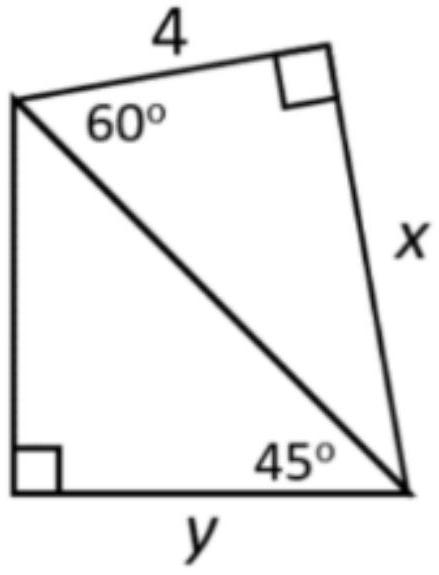
\includegraphics[max width=\textwidth, alt={}, center]{f5d7d9e6-ba61-429e-b1d7-d435782bc91b-02_575_439_296_468}

$$
\begin{aligned}
& \mathrm{x}= \\
& \mathrm{y}=
\end{aligned}
$$

A car is driving in a circular pattern on a track with a radius of 800 feet. An analyst draws a central angle with rays that intersect points corresponding to the car's initial position and its position after 40 seconds. If the angle has a measure of $\frac{13 \pi}{10}$, what is the car's average velocity (in feet per second) over the first 40 seconds? Write your answer as an exact value in simplest form.

Which of the following angles have the same reference angle? Select all that apply.\\
a) $\frac{7 \pi}{6}$\\
b) $\frac{11 \pi}{4}$\\
d) $-\frac{16 \pi}{6}$\\
e) $740^{\circ}$\\
f) $-\frac{19 \pi}{9}$\\
C) $\frac{20 \pi}{18}$\\
g) $\frac{5 \pi}{7}$\\
h) $400^{\circ}$

\begin{enumerate}
  \item Evaluate each trigonometric expression (1 point each)
\end{enumerate}

\begin{center}
\begin{tabular}{|l|l|l|}
\hline
$\sin \left(90^{\circ}\right)$ & $\sec \left(300^{\circ}\right)$ & $\tan \left(\frac{5 \pi}{4}\right)$ \\
\hline
$\csc \left(-\frac{\pi}{6}\right)$ & $\cos \left(-135^{\circ}\right)$ & $\sec \left(225^{\circ}\right)$ \\
\hline
$\cos \left(\frac{11 \pi}{4}\right)$ & $\cot \left(\frac{5 \pi}{2}\right)$ & $\sin \left(-\frac{5 \pi}{3}\right)$ \\
\hline
\end{tabular}
\end{center}

\begin{enumerate}
  \setcounter{enumi}{1}
  \item If $\tan (\theta)=\frac{2}{9}$ and $\sec (\theta)<0$ what is $\sin (\theta)$ ?\\
(2 points)
\end{enumerate}

Put the following in order from least to greatest: (3 points)\\
$\sin \left(\frac{8 \pi}{3}\right), \cos (7 \pi), \cos (10 \pi), \cos \left(-\frac{5 \pi}{3}\right), \tan \left(\frac{\pi}{6}\right), \cos \left(\frac{\pi}{13}\right)$

Greatest\\
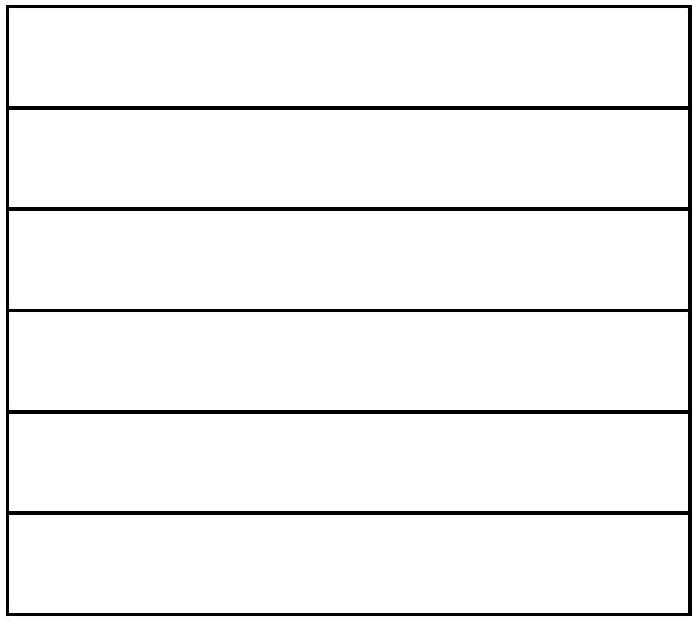
\includegraphics[max width=\textwidth, alt={}, center]{f5d7d9e6-ba61-429e-b1d7-d435782bc91b-03_624_700_1882_1228}

Least

Part 1: Fill in the $1^{\text {st }}$ quadrant of the unit circle. For each angle, indicate both degrees and radians. Also, include each ordered pair $(x, y)$ for the indicated angles (3 points)\\
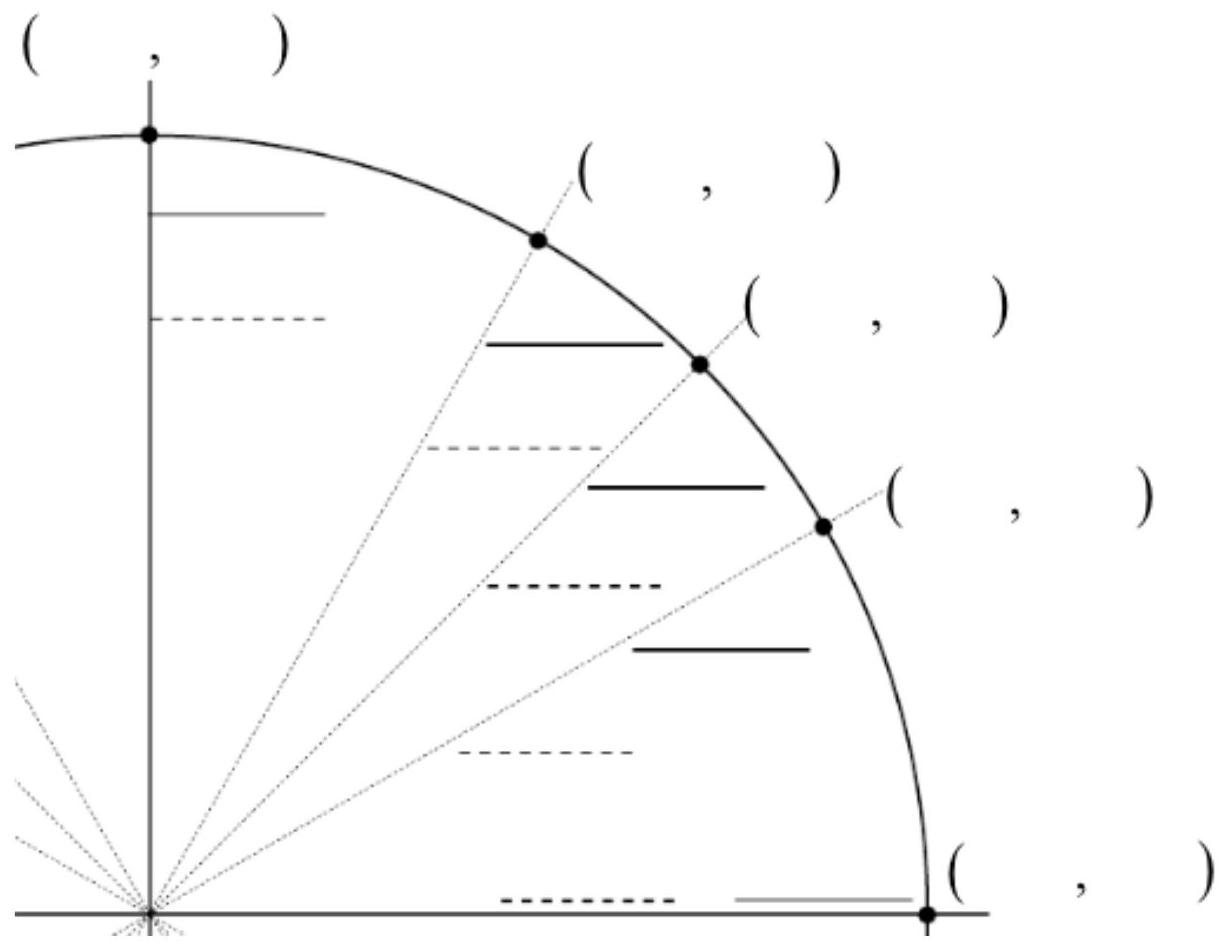
\includegraphics[max width=\textwidth, alt={}, center]{f5d7d9e6-ba61-429e-b1d7-d435782bc91b-04_952_1228_363_556}

Part 2: If $\sin (\theta)=0.915$, find each of the following (assume $\theta$ is measured in degrees) ( 1 point each)\\
a) $\sec \left(90^{\circ}-\theta\right)$\\
b) $\sin (-\theta)$\\
c) $\cos \left(\theta-90^{\circ}\right)$\\
d) $\csc (\theta)$

\begin{center}
\begin{tabular}{|l|l|}
\hline
Convert $\frac{7 \pi}{10}$ to degrees (1 point) & Convert $500^{\circ}$ to radians (1 point) \\
\hline
\multicolumn{2}{|l|}{Find two coterminal angles (one positive and one negative) for $\frac{7 \pi}{5}$ (1 point each)} \\
\hline
Positive & Negative \\
\hline
\multicolumn{2}{|c|}{\begin{tabular}{l}
Sketch each angle and then state the quadrant (or axis) in which the terminal side resides (3 points each) \( -\frac{5 \pi}{8} \) \\
3 radians \\
$\longleftrightarrow$ \\
Quadrant: \\
Quadrant: \\
\end{tabular}} \\
\hline
\multicolumn{2}{|l|}{\begin{tabular}{l}
Determine the reference angle for each. Your answer should match the form given (1 point each) \\
$-105^{\circ}$ \\
$\frac{10 \pi}{9}$ \\
$\frac{21 \pi}{8}$ \\
\end{tabular}} \\
\hline
\end{tabular}
\end{center}

\section*{Unit 6 Assessment ALL ANSWERS MUST BE SIMPLIFIED \_ Name/Date:}
Find the exact values of x and y in the diagram shown.\\
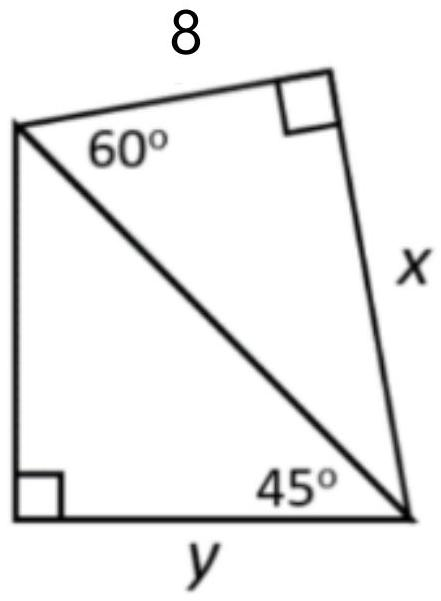
\includegraphics[max width=\textwidth, alt={}, center]{f5d7d9e6-ba61-429e-b1d7-d435782bc91b-06_601_441_270_466}

$$
\begin{aligned}
& x= \\
& y=
\end{aligned}
$$

A car is driving in a circular pattern on a track with a radius of 400 feet. An analyst draws a central angle with rays that intersect points corresponding to the car's initial position and its position after 40 seconds. If the angle has a measure of $\frac{13 \pi}{20}$, what is the car's average velocity (in feet per second) over the first 40 seconds? Write your answer as an exact value in simplest form.

Which of the following angles have the same reference angle? Select all that apply.\\
a) $-\frac{19 \pi}{9}$\\
b) $\frac{7 \pi}{6}$\\
c) $740^{\circ}$\\
d) $\frac{20 \pi}{18}$\\
e) $400^{\circ}$\\
f) $\frac{5 \pi}{7}$\\
g) $\frac{11 \pi}{4}$\\
h) $-\frac{16 \pi}{6}$

\begin{enumerate}
  \item Evaluate each trigonometric expression (1 point each)
\end{enumerate}

\begin{center}
\begin{tabular}{|l|l|l|}
\hline
$\sin \left(\mathbf{2 7 0}^{\circ}\right)$ & $\sec \left(330^{\circ}\right)$ & $\tan \left(\frac{3 \pi}{4}\right)$ \\
\hline
$\csc \left(-\frac{\pi}{\mathbf{3}}\right)$ & $\cos \left(135^{\circ}\right)$ & $\sec \left(-225^{\circ}\right)$ \\
\hline
$\cos \left(\frac{\mathbf{7} \pi}{\mathbf{4}}\right)$ & $\cot \left(\frac{9 \pi}{2}\right)$ & $\sin \left(-\frac{5 \pi}{6}\right)$ \\
\hline
\end{tabular}
\end{center}

\begin{enumerate}
  \setcounter{enumi}{1}
  \item If $\tan (\theta)=\frac{2}{7}$ and $\sec (\theta)<0$ what is $\sin (\theta)$ ?\\
(2 points)
\end{enumerate}

Put the following in order from least to greatest: (3 points)\\
$\sin \left(\frac{7 \pi}{3}\right), \cos (21 \pi), \cos (12 \pi), \cos \left(-\frac{5 \pi}{3}\right), \tan \left(\frac{\pi}{6}\right), \cos \left(\frac{\pi}{13}\right)$

Greatest\\
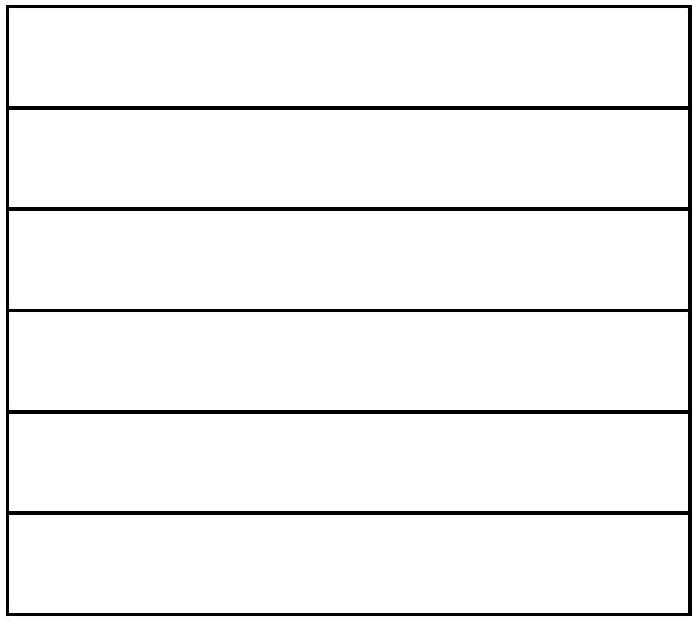
\includegraphics[max width=\textwidth, alt={}, center]{f5d7d9e6-ba61-429e-b1d7-d435782bc91b-07_624_700_1882_1228}

Least

Part 1: Fill in the $1^{\text {st }}$ quadrant of the unit circle. For each angle, indicate both degrees and radians. Also, include each ordered pair $(x, y)$ for the indicated angles (3 points)\\
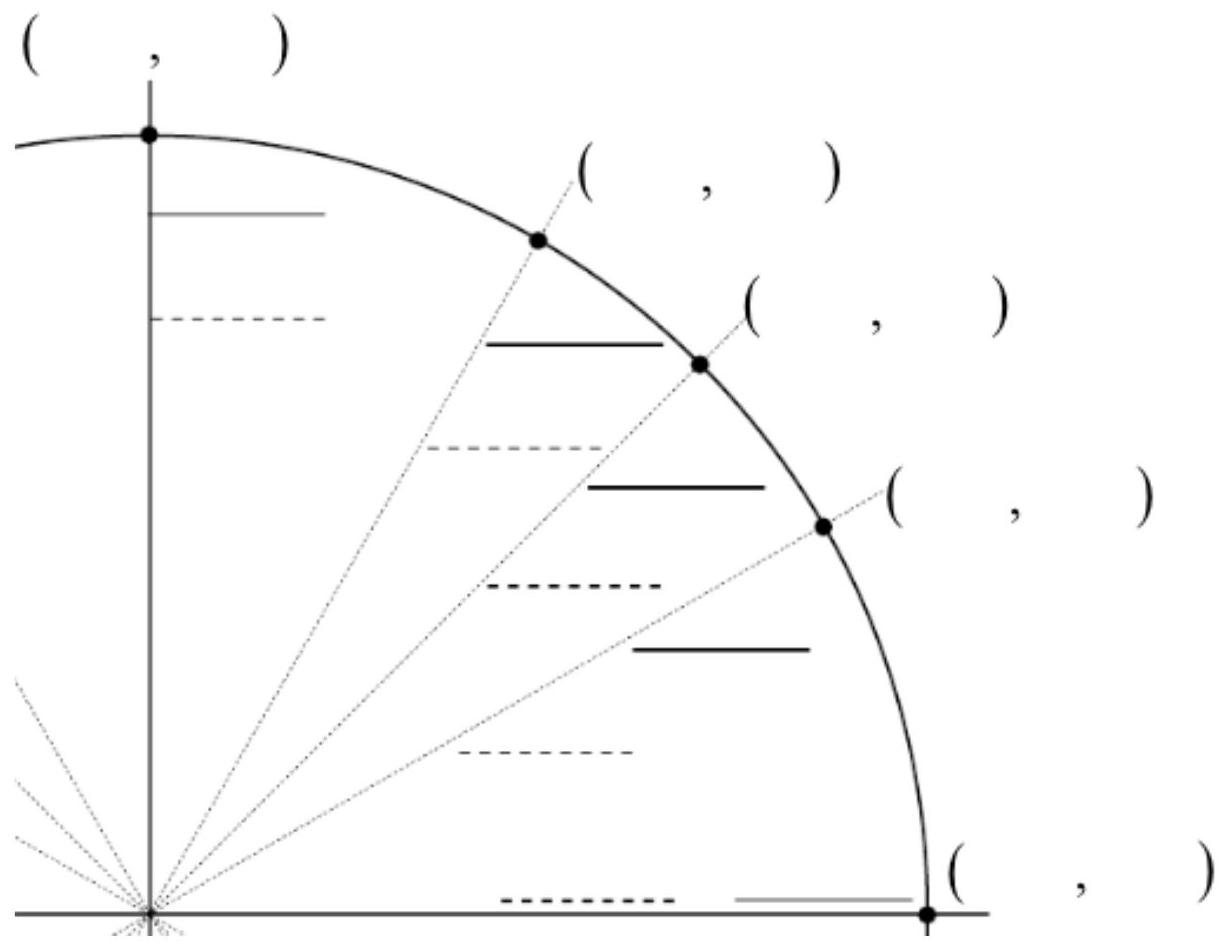
\includegraphics[max width=\textwidth, alt={}, center]{f5d7d9e6-ba61-429e-b1d7-d435782bc91b-08_952_1228_363_556}

Part 2: If $\sin (\theta)=-0.715$, find each of the following (assume $\theta$ is measured in degrees) ( 1 point each)\\
a) $\sec \left(90^{\circ}-\theta\right)$\\
b) $\sin (-\theta)$\\
c) $\cos \left(\theta-90^{\circ}\right)$\\
d) $\csc (\theta)$

\begin{center}
\begin{tabular}{|l|l|l|}
\hline
Convert $\frac{7 \pi}{12}$ to degrees (1 point) &  & Convert $490^{\circ}$ to radians (1 point) \\
\hline
\multicolumn{3}{|l|}{Find two coterminal angles (one positive and one negative) for $\frac{3 \pi}{11}$ ( 1 point each)} \\
\hline
Positive &  &  \\
\hline
\multicolumn{3}{|l|}{\begin{tabular}{l}
Sketch each angle and then state the quadrant (or axis) in which the terminal side resides (3 points each) \( -\frac{5 \pi}{8} \) \\
7 radians \\
$\longleftrightarrow$ \\
Quadrant: \\
Quadrant: \\
\end{tabular}} \\
\hline
\multicolumn{3}{|c|}{Determine the reference angle for each. Your answer should match the form given (1 point each)} \\
\hline
\end{tabular}
\end{center}

\section*{Unit 6 Assessment ALL ANSWERS MUST BE SIMPLIFIED \_ Name/Date:}
Find the exact values of x and y in the diagram shown.\\
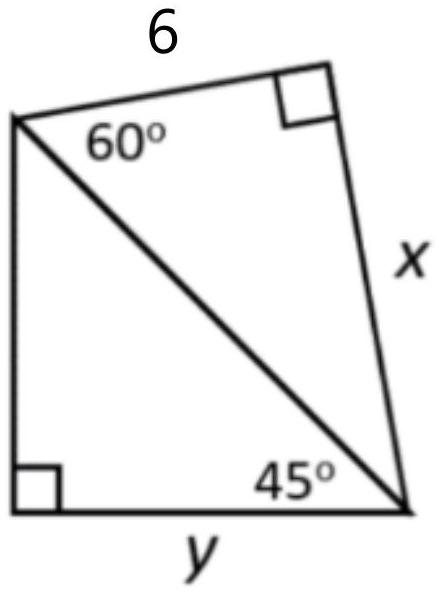
\includegraphics[max width=\textwidth, alt={}, center]{f5d7d9e6-ba61-429e-b1d7-d435782bc91b-10_594_439_277_468}

$$
\begin{aligned}
& \mathrm{x}= \\
& \mathrm{y}=
\end{aligned}
$$

A car is driving in a circular pattern on a track with a radius of 1000 feet. An analyst draws a central angle with rays that intersect points corresponding to the car's initial position and its position after 50 seconds. If the angle has a measure of $\frac{17 \pi}{10}$, what is the car's average velocity (in feet per second) over the first 50 seconds? Write your answer as an exact value in simplest form.

Which of the following angles have the same reference angle? Select all that apply.\\
a) $\frac{7 \pi}{6}$\\
b) $\frac{11 \pi}{4}$\\
d) $-\frac{16 \pi}{6}$\\
e) $740^{\circ}$\\
f) $-\frac{19 \pi}{9}$\\
C) $\frac{20 \pi}{18}$\\
g) $\frac{5 \pi}{7}$\\
h) $400^{\circ}$

\begin{enumerate}
  \item Evaluate each trigonometric expression (1 point each)
\end{enumerate}

\begin{center}
\begin{tabular}{|l|l|l|}
\hline
$\boldsymbol{\operatorname { c o s }}\left(90^{\circ}\right)$ & $\csc \left(300^{\circ}\right)$ & $\cot \left(\frac{5 \pi}{4}\right)$ \\
\hline
$\sec \left(-\frac{\pi}{6}\right)$ & $\sin \left(-135^{\circ}\right)$ & $\sec \left(-225^{\circ}\right)$ \\
\hline
$\cos \left(\frac{11 \pi}{\mathbf{6}}\right)$ & $\tan \left(\frac{5 \pi}{2}\right)$ & $\sin \left(-\frac{5 \pi}{2}\right)$ \\
\hline
\end{tabular}
\end{center}

\begin{enumerate}
  \setcounter{enumi}{1}
  \item If $\tan (\theta)=-\frac{5}{9}$ and $\sec (\theta)>0$ what is $\sin (\theta) ?(2$ points)
\end{enumerate}

\section*{Put the following in order from least to greatest: (3 points)}
$\sin \left(\frac{8 \pi}{3}\right), \cos (7 \pi), \cos (-10 \pi), \cos \left(-\frac{5 \pi}{3}\right), \tan \left(\frac{\pi}{6}\right), \cos \left(\frac{\pi}{13}\right)$

\section*{Greatest}
\begin{center}
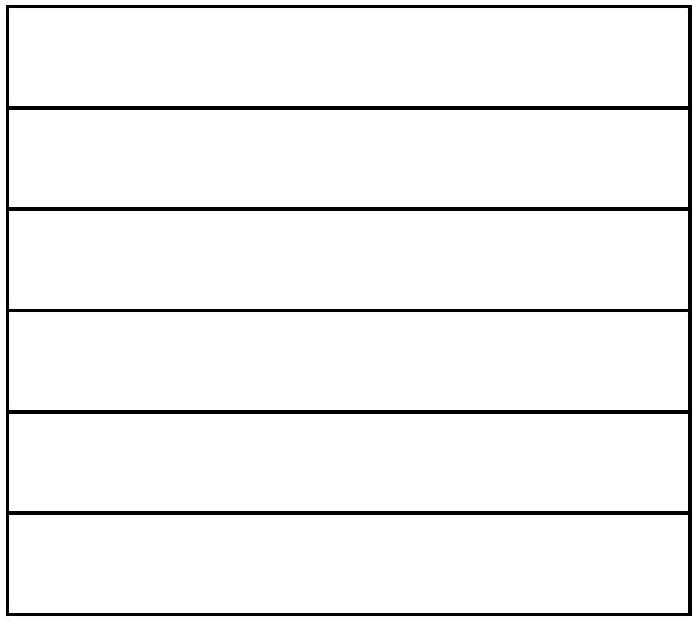
\includegraphics[max width=\textwidth, alt={}]{f5d7d9e6-ba61-429e-b1d7-d435782bc91b-11_624_700_1882_1228}
\end{center}

Least

Part 1: Fill in the $1^{\text {st }}$ quadrant of the unit circle. For each angle, indicate both degrees and radians. Also, include each ordered pair $(x, y)$ for the indicated angles (3 points)\\
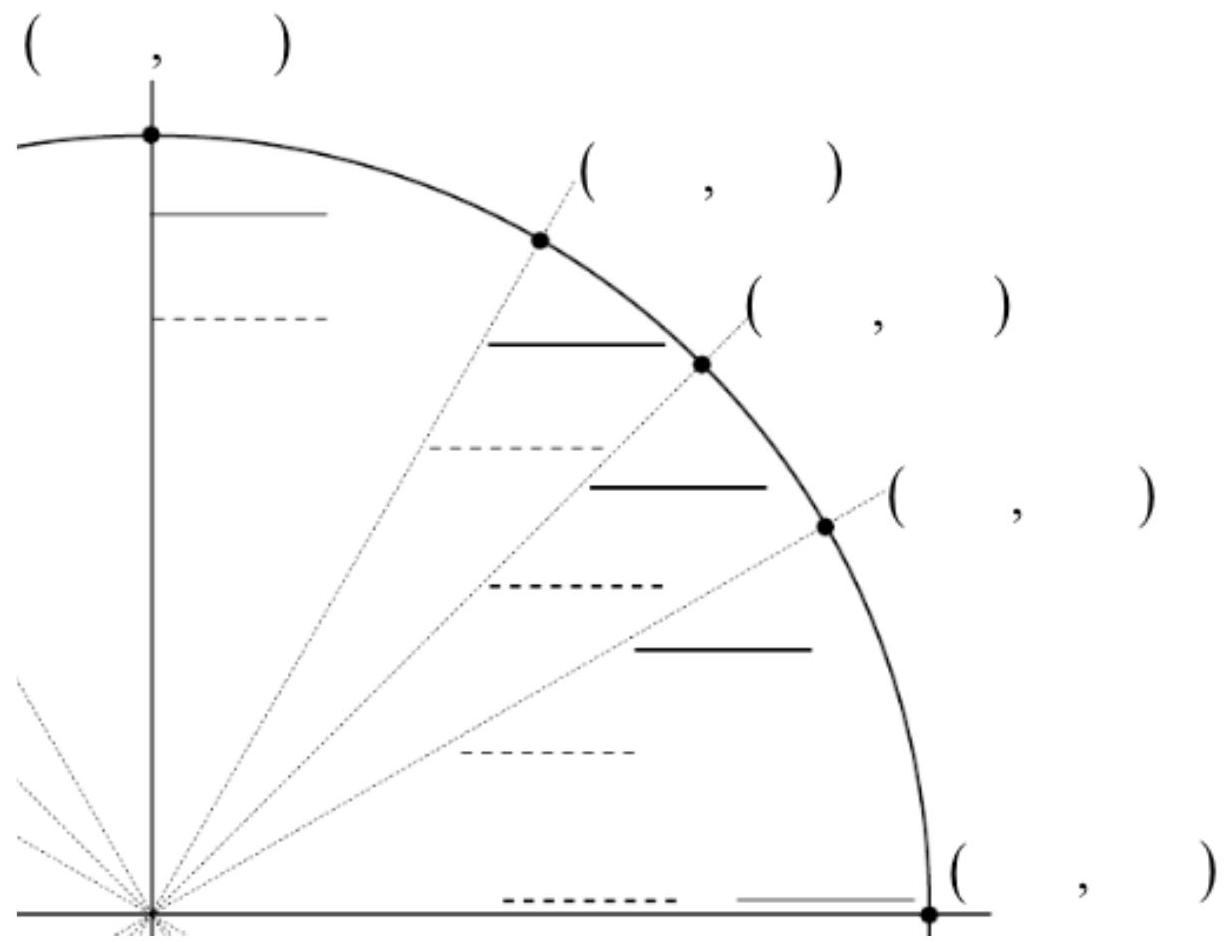
\includegraphics[max width=\textwidth, alt={}, center]{f5d7d9e6-ba61-429e-b1d7-d435782bc91b-12_952_1230_363_554}

Part 2: If $\sin (\theta)=0.615$, find each of the following (assume $\theta$ is measured in degrees) ( 1 point each)\\
a) $\sec \left(90^{\circ}-\theta\right)$\\
b) $\sin (-\theta)$\\
c) $\cos \left(\theta-90^{\circ}\right)$\\
d) $\csc (\theta)$


\end{document}